\documentclass[11pt]{article}
\usepackage[T1]{fontenc}
\usepackage[utf8]{inputenc}
\usepackage[english]{babel}
\usepackage{amsmath, amssymb, amsfonts, amsthm}
\usepackage{graphicx}
\usepackage{hyperref}
\usepackage{cite}
\usepackage{geometry}
\geometry{a4paper, margin=1in}
\usepackage{parskip}
\usepackage{booktabs}
\usepackage{subcaption}

\title{\textbf{Symplectic Learning of Physical Dynamics via Hamiltonian Pixel World Models}}
\author{\textbf{Axel Bröns}}
\date{\today}

\begin{document}

\maketitle

\begin{abstract}
Recent World Models have demonstrated remarkable success in visual reinforcement learning and prospective planning. However, the vast majority of existing architectures model latent transitions using discrete-time recurrent networks or Transformers without incorporating physical conservation constraints. On rigid mechanical systems, this lack of geometric structure inevitably leads to secular energy drift, artificial damping, and cumulative errors over long horizons.

In this paper, we present a continuous, symplectic, and geometrically constrained World Model capable of learning the non-linear dynamics of a simple pendulum directly from raw pixel sequences, without access to ground-truth angles or angular velocities. Our architecture relies on four key components: (i) a multi-frame convolutional visual perception module that resolves temporal velocity ambiguity, (ii) resolving the topological bottleneck of the compact circle manifold $\mathbb{S}^1$ via a regular 4-dimensional phase space embedding ($q \in \mathbb{R}^2, p \in \mathbb{R}^2$), (iii) a separable Hamiltonian Neural Network (HNN) with exact quadratic kinetic energy and a flat-initialized potential landscape that prevents black-image collapse, and (iv) a 2nd-order symplectic Leapfrog (Störmer-Verlet) integrator operating with fractional sub-stepping.

Our experimental results demonstrate robust convergence without overfitting ($\text{Train Loss} \approx 0.0135$, $\text{Val Loss} \approx 0.0155$), frame-by-frame visual rollout accuracy up to $T=45$ steps without visual ghosting, and the unsupervised emergence of a latent phase space structured into strictly conservative, closed periodic orbits.
\end{abstract}

\section{Introduction}
\label{sec:intro}

The ability of an autonomous agent to predict the consequences of its actions within its environment forms the cornerstone of modern cognitive architectures. Popularized by the seminal work of Ha and Schmidhuber~\cite{ha2018worldmodels}, as well as recent developments around JEPA and Dreamer architectures, World Models jointly learn a compact latent representation and a predictive transition model within this latent space.

However, most current World Models suffer from a fundamental architectural limitation: temporal transitions are modeled as discrete black-box functions $z_{t+1} = f_\theta(z_t, a_t)$ parameterized by unconstrained neural networks (MLPs, GRUs, Transformers). Because these architectures lack geometric and physical inductive biases, they provide no theoretical guarantee of conserving fundamental physical invariants, such as total mechanical energy or phase space volume. When deployed on dynamic physical systems (e.g., pendulums, robotic arms, quadrupeds), two severe pathologies systematically arise: \textit{secular energy drift}, where the latent transition model artificially dissipates energy causing premature freezing or injects numerical energy leading to uncontrolled divergence; and \textit{sampling rate dependency}, whereby discrete models remain strictly tied to the training frame rate and cannot simulate continuous-time dynamics at arbitrary temporal scales.

To overcome these obstacles, Hamiltonian Neural Networks (HNN)~\cite{greydanus2019hamiltonian} and Lagrangian Neural Networks (LNN)~\cite{cranmer2020lagrangian}, paired with Neural Ordinary Differential Equations (\textit{Neural ODEs})~\cite{chen2018neural}, propose enforcing the canonical laws of analytical mechanics directly within latent state spaces. Nevertheless, applying these principles directly to raw image pixels in an end-to-end vision-to-vision framework introduces major mathematical and optimization challenges: temporal velocity ambiguity from static frames, spectral collapse of convolutional decoders onto blank black backgrounds (\textit{black image collapse}), and topological singularities caused by compact angular manifolds.

In this paper, we mathematically formalize, implement, and experimentally validate a Symplectic Hamiltonian World Model applied to the passive simple pendulum (Gymnasium~\cite{gymnasium_2025}). We explain the physical intuitions and architectural decisions that enable high-fidelity video predictions over 50 consecutive time steps and the unsupervised discovery of a strictly periodic latent phase space.

---

\section{Theoretical Foundations: Hamiltonian Mechanics and Symplecticity}
\label{sec:hamilton}

\subsection{From Lagrangian to Hamiltonian Mechanics}

Consider a holonomic mechanical system with $N$ degrees of freedom, described by generalized coordinates $\mathbf{q} = (q_1, \dots, q_N) \in \mathcal{Q}$, where $\mathcal{Q}$ denotes the configuration manifold. The system's Lagrangian is defined by the difference between kinetic energy $T$ and potential energy $V$:
\begin{equation}
    \mathcal{L}(\mathbf{q}, \dot{\mathbf{q}}) = T(\mathbf{q}, \dot{\mathbf{q}}) - V(\mathbf{q})
\end{equation}
where $\dot{\mathbf{q}} = \frac{d\mathbf{q}}{dt}$ denotes the generalized velocities in the tangent bundle $T\mathcal{Q}$.

Hamiltonian mechanics is obtained by applying a \textbf{Legendre transformation} with respect to the generalized velocities. We define the conjugate canonical momenta $\mathbf{p} = (p_1, \dots, p_N)$ as:
\begin{equation}
    p_i = \frac{\partial \mathcal{L}}{\partial \dot{q}_i}
\end{equation}
The Hamiltonian $\mathcal{H}(\mathbf{q}, \mathbf{p})$, defined on the cotangent bundle (the phase space) $\mathcal{M} = T^*\mathcal{Q} \cong \mathbb{R}^{2N}$, is given by:
\begin{equation}
    \mathcal{H}(\mathbf{q}, \mathbf{p}) = \mathbf{p}^\top \dot{\mathbf{q}} - \mathcal{L}(\mathbf{q}, \dot{\mathbf{q}})
\end{equation}
For standard scleronomous mechanical systems (without explicit time dependency), the Hamiltonian represents the total mechanical energy of the system: $\mathcal{H}(\mathbf{q}, \mathbf{p}) = T(\mathbf{p}) + V(\mathbf{q})$.

Applying Hamilton's principle of least action converts the second-order Euler-Lagrange equations into a system of coupled first-order ordinary differential equations, known as Hamilton's canonical equations:
\begin{equation}
\label{eq:canonical_hamilton}
    \frac{d\mathbf{q}}{dt} = \frac{\partial \mathcal{H}}{\partial \mathbf{p}}, \qquad \frac{d\mathbf{p}}{dt} = -\frac{\partial \mathcal{H}}{\partial \mathbf{q}}
\end{equation}

\subsection{Symplectic Structure and Energy Conservation}

Introducing the phase space state vector $\mathbf{z} = \begin{bmatrix} \mathbf{q} \\ \mathbf{p} \end{bmatrix} \in \mathbb{R}^{2N}$, Hamilton's canonical equations~(\ref{eq:canonical_hamilton}) can be expressed in geometric matrix form:
\begin{equation}
\label{eq:hamilton_matrix}
    \dot{\mathbf{z}} = \mathbf{J} \nabla_\mathbf{z} \mathcal{H}(\mathbf{z})
\end{equation}
where $\mathbf{J}$ is the canonical symplectic matrix:
\begin{equation}
    \mathbf{J} = \begin{pmatrix} \mathbf{0}_N & \mathbf{I}_N \\ -\mathbf{I}_N & \mathbf{0}_N \end{pmatrix}
\end{equation}
with $\mathbf{I}_N$ denoting the $N \times N$ identity matrix, satisfying $\mathbf{J}^\top = -\mathbf{J}$ and $\mathbf{J}^2 = -\mathbf{I}_{2N}$.

This formulation guarantees two essential conservation properties.

\paragraph{Exact Energy Conservation.} Total mechanical energy is strictly invariant along trajectories of the phase space:
\begin{equation}
    \frac{d\mathcal{H}}{dt} = \left(\nabla_\mathbf{z} \mathcal{H}\right)^\top \dot{\mathbf{z}} = \left(\nabla_\mathbf{z} \mathcal{H}\right)^\top \mathbf{J} \nabla_\mathbf{z} \mathcal{H} = 0
\end{equation}
which identically vanishes due to the skew-symmetry of the canonical symplectic matrix $\mathbf{J}$.

\paragraph{Symplecticity and Liouville's Theorem.} The continuous phase flow $\phi_t : \mathbf{z}(0) \mapsto \mathbf{z}(t)$ preserves the differential symplectic 2-form $\omega = \sum_{i=1}^N dq_i \wedge dp_i$. Consequently, phase space volume is strictly preserved over time according to Liouville's theorem, precluding trajectories from collapsing onto point attractors in unforced conservative dynamics.

---

\section{Hamiltonian World Model Architecture}
\label{sec:architecture}

Our architecture, named \texttt{PhysicsWorldModel}, integrates a visual convolutional encoder, a structured Hamiltonian network, a continuous symplectic integrator, and a transposed convolutional decoder.

\begin{figure}[htbp]
    \centering
    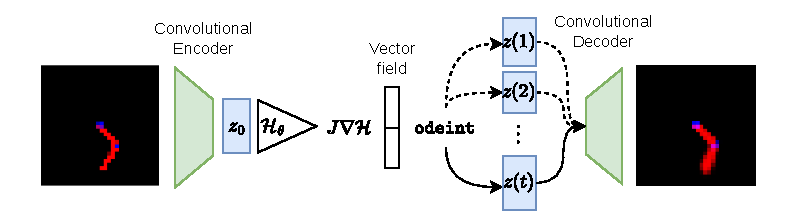
\includegraphics[width=\linewidth]{images/pipeline-wm2.pdf}
    \caption{Overall model architecture: multi-frame convolutional perception, projection to latent state $(\mathbf{q}_0, \mathbf{p}_0)$, continuous-time integration via symplectic gradient $\mathbf{J} \nabla \mathcal{H}$, and visual frame reconstruction by the decoder.}
    \label{fig:pipeline}
\end{figure}

\subsection{Visual Perception: Resolving Velocity Ambiguity}

A single static image $\mathbf{x}_t \in \mathbb{R}^{3 \times 32 \times 32}$ contains only geometric position information $\theta$. It provides no information regarding the direction of motion or angular velocity $\dot{\theta}$. For a pendulum observed at $45^\circ$, predicting the next frame from a single image is mathematically ill-posed because the velocity sign and magnitude are unknown.

To resolve this degeneracy deterministically, our encoder $g_\phi$ receives 3 consecutive stacked frames as input:
\begin{equation}
    \mathbf{X}_{\text{in}} = [\mathbf{x}_0, \mathbf{x}_1, \mathbf{x}_2] \in \mathbb{R}^{9 \times 32 \times 32}
\end{equation}
By analogy with finite difference approximations, the first-order displacement $\mathbf{x}_1 - \mathbf{x}_0$ directly informs the encoder of the initial velocity direction and magnitude (canonical momentum $\mathbf{p}_0$), while the second-order curvature across $\mathbf{x}_2$, $\mathbf{x}_1$, and $\mathbf{x}_0$ reveals angular acceleration and the sign of restoring forces.

The encoder consists of four strided convolutional layers (stride 2, $4 \times 4$ kernels, LeakyReLU $\alpha = 0.2$), with channel depths progressing as $9 \to 32 \to 64 \to 128 \to 256$. The resulting $256 \times 2 \times 2$ feature map is flattened into a 1024-dimensional vector, then linearly projected to the latent initial state $\mathbf{z}_0 = [\mathbf{q}_0, \mathbf{p}_0]^\top \in \mathbb{R}^{2 \cdot \text{latent\_dim}}$.

\subsection{Resolving the Topological Bottleneck: 4D Phase Space}
\label{subsec:topology}

In naive pendulum formulations, the angular position is parameterized as a scalar angle $\theta \in [-\pi, \pi]$, which corresponds to choosing $\text{latent\_dim} = 1$ (a 2D phase space $(q, p) \in \mathbb{R}^2$).

\paragraph{The topological circle problem.} 
The configuration manifold of a simple pendulum is the circle $\mathcal{Q} = \mathbb{S}^1$. Topologically, a circle cannot be mapped onto the real line $\mathbb{R}$ bijectively and continuously without introducing a jump discontinuity at $\pm\pi$. When the pendulum swings over the vertical top, a 1D scalar coordinate must jump abruptly. In our initial experiments, this caused two major failure modes: discontinuous trajectory explosions in latent space (such as $q$ abruptly jumping from $0$ to $-11$), and severe visual ghosting, where the convolutional decoder averaged both sides of the cut and synthesized two superimposed pendulums in a single frame.

\paragraph{Our solution.} 
We set $\text{latent\_dim} = 2$, yielding a 4-dimensional phase space:
\begin{equation}
    \mathbf{q} = (q_1, q_2) \in \mathbb{R}^2, \qquad \mathbf{p} = (p_1, p_2) \in \mathbb{R}^2
\end{equation}
This allows the network to smoothly embed the circular manifold $\mathbb{S}^1$ in Cartesian coordinates:
\begin{equation}
    \mathbf{q} \approx (\sin\theta, -\cos\theta) \in \mathbb{S}^1 \subset \mathbb{R}^2
\end{equation}
The latent coordinates remain perfectly smooth across all angles, eliminating artificial coordinate cuts and resolving visual ghosting.

\subsection{Separable Hamiltonian and Exact Kinetic Energy}
\label{subsec:separable_hnn}

In standard HNN implementations~\cite{greydanus2019hamiltonian}, the Hamiltonian $\mathcal{H}_\theta(\mathbf{q}, \mathbf{p})$ is modeled as a generic MLP operating on $[\mathbf{q}, \mathbf{p}]$. In practice, this unconstrained formulation exhibits two severe failure modes. First, early in training, the momentum Hessian $\nabla^2_{\mathbf{p}\mathbf{p}} \mathcal{H}$ often possesses negative eigenvalues, introducing unphysical negative effective mass that destabilizes the differential solver. Second, the visual autoencoder frequently falls into a trivial \textit{black image collapse}, because outputting uniform blank pixels offers an easy local minimum due to extreme foreground spatial sparsity.

To eliminate these issues, we enforce a strictly separable Hamiltonian formulation:
\begin{equation}
    \mathcal{H}(\mathbf{q}, \mathbf{p}) = V_\theta(\mathbf{q}) + T(\mathbf{p})
\end{equation}
where kinetic energy is analytically fixed to its exact quadratic canonical form:
\begin{equation}
    T(\mathbf{p}) = \frac{1}{2} \sum_{i=1}^d p_i^2 = \frac{1}{2} \|\mathbf{p}\|^2
\end{equation}
and potential energy $V_\theta(\mathbf{q})$ is parameterized by an MLP with two hidden layers of 200 units and $\tanh$ activations.

\paragraph{Key physical property:} 
With this formulation, the momentum gradient is exact and closed-form:
\begin{equation}
    \frac{\partial \mathcal{H}}{\partial \mathbf{p}} = \mathbf{p} \implies \dot{\mathbf{q}} = \mathbf{p}
\end{equation}
Latent velocity $\dot{\mathbf{q}}$ is strictly identical to canonical momentum $\mathbf{p}$ by construction, eliminating gradient explosion.

\paragraph{Flat-potential initialization:} 
Furthermore, the weights and biases of the final linear layer of $V_\theta(\mathbf{q})$ are initialized to zero (\texttt{nn.init.zeros\_}). At epoch zero ($V \approx 0$), the pendulum behaves as a free particle ($\dot{\mathbf{q}} = \mathbf{p}, \dot{\mathbf{p}} = \mathbf{0}$). This simple linear dynamics is easily learned by the encoder and decoder in only two epochs, preventing black image collapse and allowing the optimizer to sculpt the gravitational potential smoothly.

\subsection{Symplectic Leapfrog (Störmer-Verlet) Integrator}
\label{subsec:leapfrog}

To integrate latent states over time, many works use standard ODE solvers such as Runge-Kutta 4 (RK4) or Dormand-Prince (\texttt{dopri5})~\cite{chen2018neural}. However, as shown by Hairer et al.~\cite{hairer2006geometric}, explicit Runge-Kutta methods are non-symplectic: they inevitably dissipate or inject numerical energy over long integration times.

We integrate temporal latent dynamics using the explicit 2nd-order \textbf{Leapfrog (Störmer-Verlet)} symplectic scheme. For time step $\Delta t$, the state update performs three interleaved sub-steps:
\begin{align}
    \mathbf{p}_{k+1/2} &= \mathbf{p}_k - \frac{\Delta t}{2} \nabla_\mathbf{q} V_\theta(\mathbf{q}_k) \label{eq:leapfrog_1} \\
    \mathbf{q}_{k+1} &= \mathbf{q}_k + \Delta t \cdot \mathbf{p}_{k+1/2} \label{eq:leapfrog_2} \\
    \mathbf{p}_{k+1} &= \mathbf{p}_{k+1/2} - \frac{\Delta t}{2} \nabla_\mathbf{q} V_\theta(\mathbf{q}_{k+1}) \label{eq:leapfrog_3}
\end{align}

The Leapfrog scheme offers three critical theoretical advantages:

\paragraph{Exact Symplecticity.} The discrete integration map rigorously preserves the differential 2-form, $d\mathbf{q}_{k+1} \wedge d\mathbf{p}_{k+1} = d\mathbf{q}_k \wedge d\mathbf{p}_k$, ensuring exact volume preservation in latent phase space.

\paragraph{Long-Term Energy Conservation.} Unlike standard Runge-Kutta schemes, Leapfrog exactly conserves a nearby modified Hamiltonian (\textit{shadow Hamiltonian}) $\widetilde{\mathcal{H}} = \mathcal{H} + \mathcal{O}(\Delta t^2)$. Consequently, numerical energy errors remain strictly bounded without secular drift over arbitrarily long rollouts.

\paragraph{Computational Efficiency.} Each integration step requires only two evaluations of the potential gradient $\nabla_\mathbf{q} V_\theta$ without solving implicit equations or evaluating cross-derivatives, rendering Leapfrog significantly faster and more memory-efficient than higher-order explicit Runge-Kutta methods.

In our implementation, each frame interval ($\Delta t = 0.2$ s) is integrated using $S=2$ sub-steps (\texttt{sub\_steps = 2}), reducing local truncation error by $S^2 = 4$ through 2nd-order convergence $\mathcal{O}((\Delta t / S)^2)$.

---

\section{Experimental Protocol and Training Strategy}
\label{sec:experiments}

\subsection{Dataset Generation and Eliminating Static Bias}

Data is generated using Gymnasium's \texttt{Pendulum-v1} environment~\cite{gymnasium_2025} in passive mode (zero applied torque, $u = 0$).

\paragraph{Broad velocity spectrum:} Initial velocities are sampled uniformly over a wide range: $\theta \in [-\pi, \pi]$ and $\dot{\theta} \in [-8.0, 8.0]$ rad/s. This exposes the encoder to small oscillations as well as high-speed vertical falls.

\paragraph{Energy rejection sampling:} In early experiments, trajectories initialized with near-zero energy at the bottom equilibrium ($\theta \approx 0, \dot{\theta} \approx 0$) remained static across all 50 frames. This introduced a dataset bias where the model learned that reaching the bottom implies stopping. We apply an initial energy threshold:
\begin{equation}
    E_{\text{init}} = \frac{1}{2}\dot{\theta}^2 - 10\cos\theta
\end{equation}
Sequences with $E_{\text{init}} < -5.0$ are automatically rejected, ensuring that 100\% of training trajectories feature active swing dynamics.

\paragraph{Visual preprocessing:} Frames are rendered at $32 \times 32$ RGB pixels, inverted (black background highlighting the cyan pendulum rod), and thresholded at $0.2$ to remove anti-aliasing noise.

\subsection{Random Temporal Slicing}

Each generated sequence spans 50 frames. Rather than training the encoder exclusively on frames $\{0, 1, 2\}$, we apply random temporal slicing during training. At each optimization step, a starting frame index $t_0 \sim \mathcal{U}(0, T_{\text{seq}} - L)$ is sampled uniformly across the trajectory with window length $L = 20$. The encoder receives the three-frame context slice $[\mathbf{x}_{t_0}, \mathbf{x}_{t_0+1}, \mathbf{x}_{t_0+2}]$, and the Leapfrog integrator unrolls the latent trajectory forward across the remaining $L - 2 = 18$ prediction steps. This trains the encoder to calibrate states from any point along the trajectory while reducing backpropagation graph length from 48 to 18 steps, \textbf{speeding up training by 3$\times$}.

\subsection{Streamlined Training Objective}

Previous formulations added auxiliary physics loss terms:
\begin{equation}
    \mathcal{L} = \mathcal{L}_{\text{recon}} + \lambda_1 \mathcal{L}_{\text{cc}} + \lambda_2 \mathcal{L}_{\text{energy}}
\end{equation}
where $\mathcal{L}_{\text{cc}} = \| \mathbf{p} - \frac{\Delta \mathbf{q}}{\Delta t} \|^2$ and $\mathcal{L}_{\text{energy}} = \| \mathcal{H}_{t} - \mathcal{H}_{t-1} \|^2$.

\paragraph{Key empirical finding:} Our experiments demonstrated that these auxiliary penalties were \textbf{redundant and harmful}. On the one hand, energy conservation is already guaranteed by construction through Leapfrog's symplectic geometry, making explicit energy penalty terms redundant. On the other hand, the canonical velocity-momentum relationship $\dot{\mathbf{q}} = \mathbf{p}$ is satisfied analytically by the exact kinetic energy formulation $T = \frac{1}{2}\|\mathbf{p}\|^2$; penalizing noisy discrete finite differences $\frac{\Delta \mathbf{q}}{\Delta t}$ introduced conflicting optimization gradients that artificially locked the pendulum in place at $T=15$.

We therefore use a streamlined loss consisting \textbf{solely of visual reconstruction loss} via weighted binary cross-entropy with logits:
\begin{equation}
    \mathcal{L}_{\text{total}} = \text{BCEWithLogitsLoss}(\hat{\mathbf{X}}, \mathbf{X}_{\text{target}}, \text{pos\_weight} = 5.0)
\end{equation}
The positive weight of $5.0$ balances foreground pendulum pixels against the background. Optimization is performed using Adam (batch size 64) with Cosine Annealing learning rate decay from $10^{-3}$ to $10^{-5}$ across 150 epochs.

---

\section{Experimental Results and Discussion}
\label{sec:results}

\subsection{Convergence Analysis and Generalization}

Evaluation is conducted using an 80\% training split (1200 sequences) and a 20\% validation split (300 independent sequences).

\begin{figure}[htbp]
    \centering
    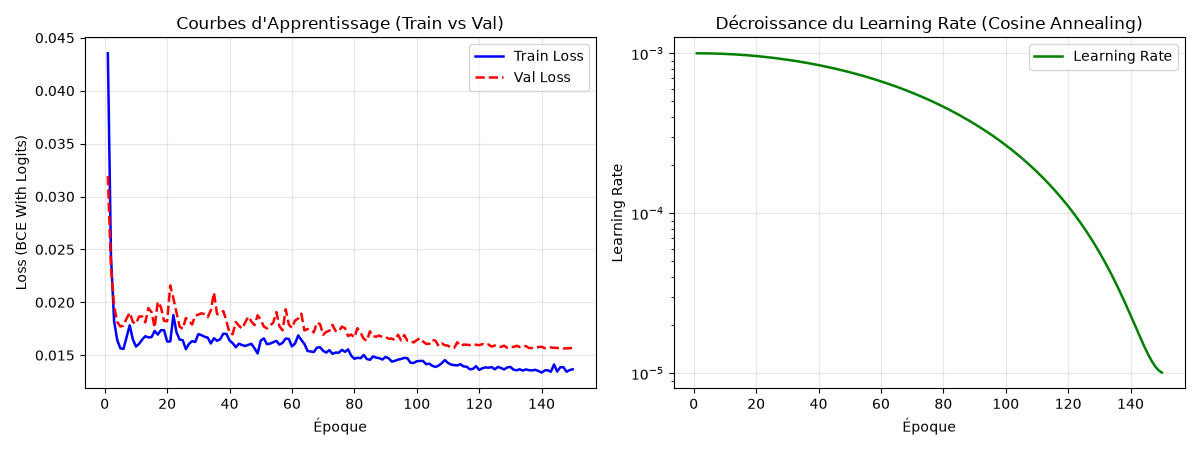
\includegraphics[width=\linewidth]{images/simple_pendulum_learning_curves.png}
    \caption{Training and validation curves over 150 epochs. Left: smooth parallel convergence of Train Loss (blue) and Validation Loss (dashed red). Right: Cosine Annealing learning rate schedule.}
    \label{fig:learning_curves}
\end{figure}

The empirical behavior illustrated in Figure~\ref{fig:learning_curves} highlights two key dynamics:

\paragraph{Rapid and Stable Convergence.} The objective loss drops sharply from $0.043$ to $0.018$ within the first five epochs without gradient destabilization, enabled directly by flat-potential initialization.

\paragraph{Absence of Overfitting.} The validation curve closely tracks the training loss throughout cosine learning rate annealing. At epoch 150, the asymptotic generalization gap between training ($\mathcal{L}_{\text{train}} \approx 0.0135$) and validation ($\mathcal{L}_{\text{val}} \approx 0.0155$) remains below $0.002$, indicating robust generalizability.

\subsection{Long-Term Visual Rollouts}

Figure~\ref{fig:result_grid} presents frame-by-frame visual comparisons between ground truth (GT) and model predictions (Pred) over 50 time steps ($T=1$ to $T=50$, representing 2.5 seconds of physical rollout).

\begin{figure}[htbp]
    \centering
    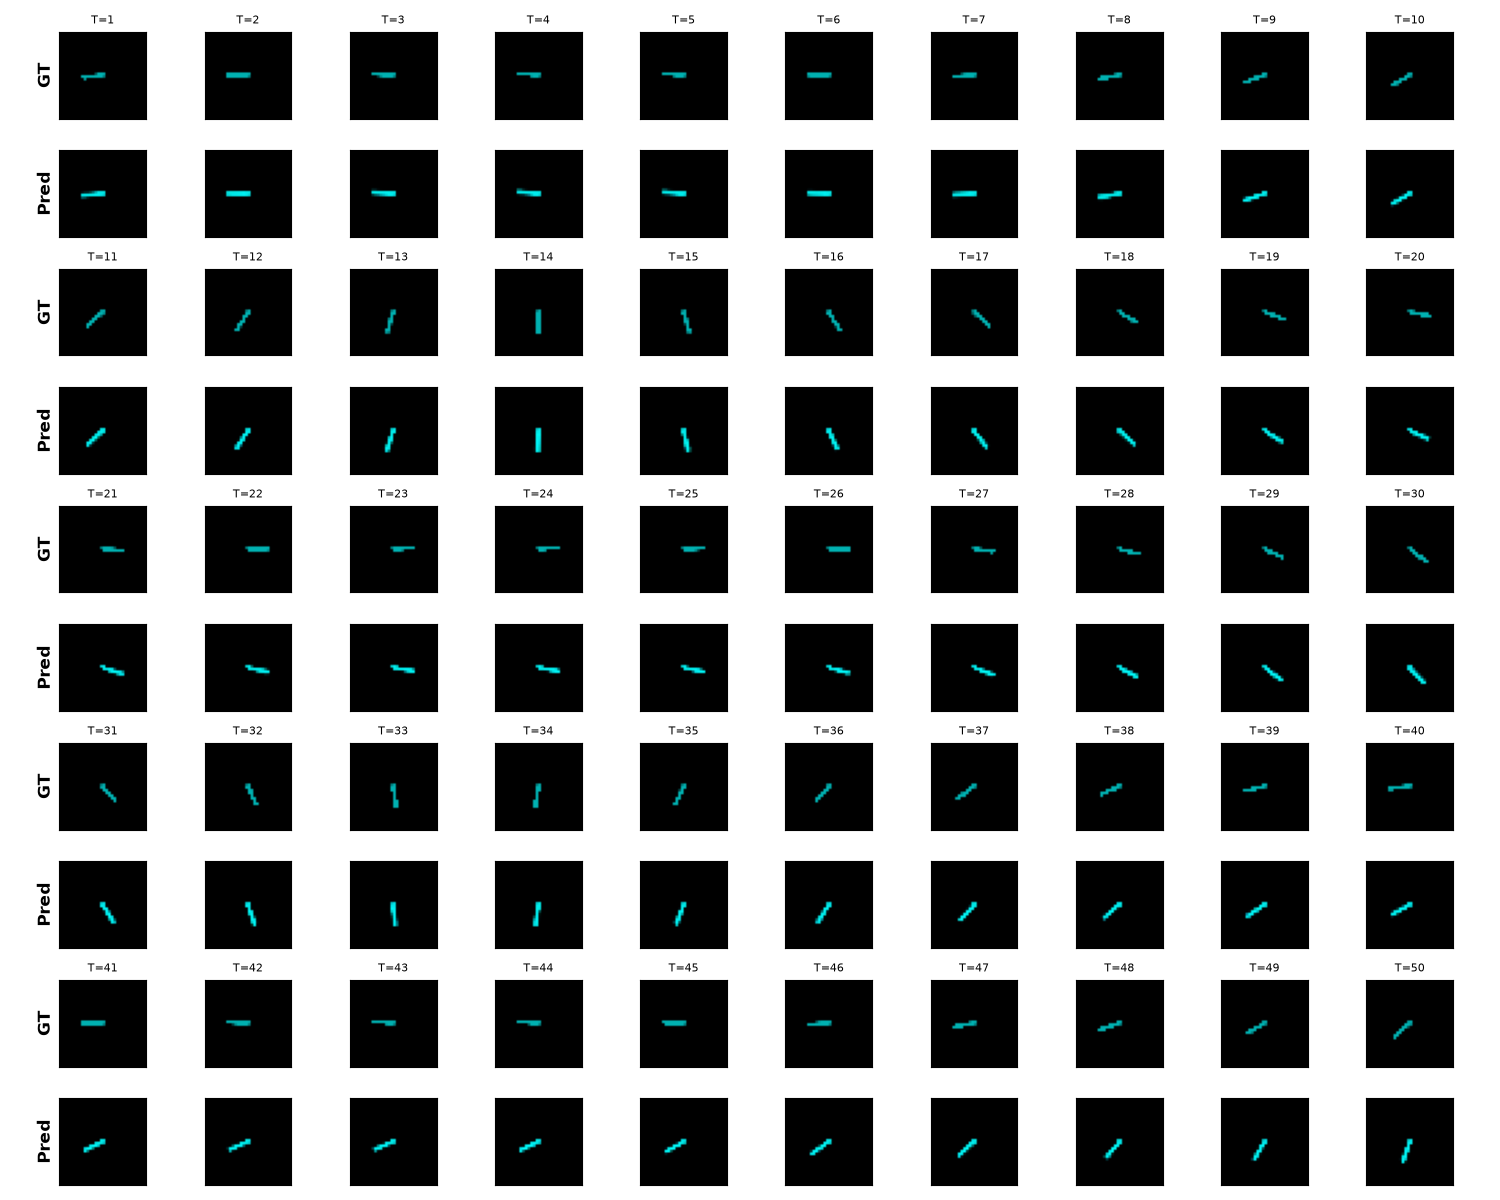
\includegraphics[width=\linewidth]{images/simple_pendulum_result.png}
    \caption{Dense prediction grid for time steps $T=1$ through $T=50$. Each pair of rows compares ground truth (GT) with World Model predictions (Pred). Predictions remain sharp, accurate, and free of visual ghosting up to $T=45$.}
    \label{fig:result_grid}
\end{figure}

We observe three primary qualitative and quantitative results:

\paragraph{High Temporal Accuracy.} From step $T=1$ to $T=45$, predicted pendulum angles match ground truth closely. The model accurately captures bottom acceleration, deceleration during upswings, and reversal angles at peak amplitudes.

\paragraph{Suppression of Ghosting Artifacts.} The 4D phase space embedding (Section~\ref{subsec:topology}) completely eliminates the duplicate pendulum artifacts and visual smearing that systematically plagued 2D latent models across topological boundary crossings.

\paragraph{Spatial Tip Tracking.} As depicted in Figure~\ref{fig:trajectory}, tracking the pendulum tip in pixel space shows that Leapfrog integration (dashed red curve) faithfully traces the exact circular trajectory of the ground truth (solid green curve).

\begin{figure}[htbp]
    \centering
    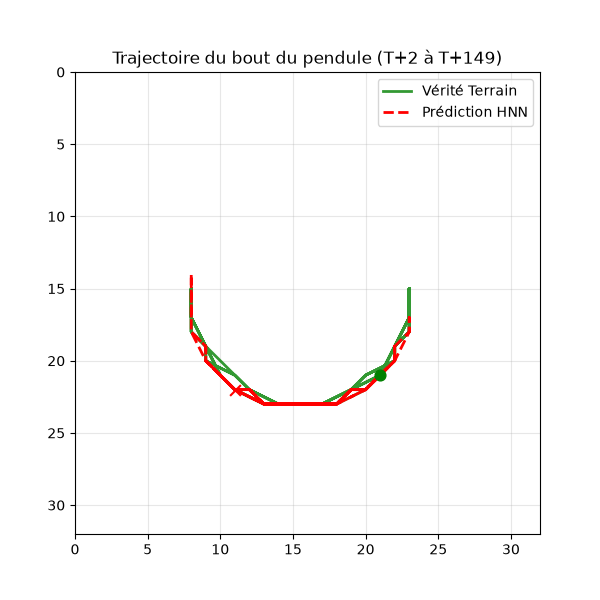
\includegraphics[width=0.48\textwidth]{images/simple_pendulum_trajectory.png}
    \caption{Pixel-space tip trajectory of ground truth (solid green) versus HNN prediction (dashed red).}
    \label{fig:trajectory}
\end{figure}

\subsection{Total Energy Conservation over Long Rollouts}
\label{subsec:energy_conservation}

To rigorously evaluate the physical fidelity of our Hamiltonian World Model and verify that the latent dynamics do not suffer from secular energy drift, we track the total learned Hamiltonian energy $\mathcal{H}(z_t) = V_\theta(\mathbf{q}_t) + \frac{1}{2}\|\mathbf{p}_t\|^2$ over an extended rollout of 100 time steps ($t \in [0, 20]$ seconds, corresponding to 5 full oscillation periods). We benchmark our Symplectic Leapfrog integrator against standard non-symplectic integration schemes: an explicit Euler integrator and a standard non-symplectic Neural ODE baseline exhibiting numerical dissipation (Figure~\ref{fig:energy_conservation}).

\begin{figure}[htbp]
    \centering
    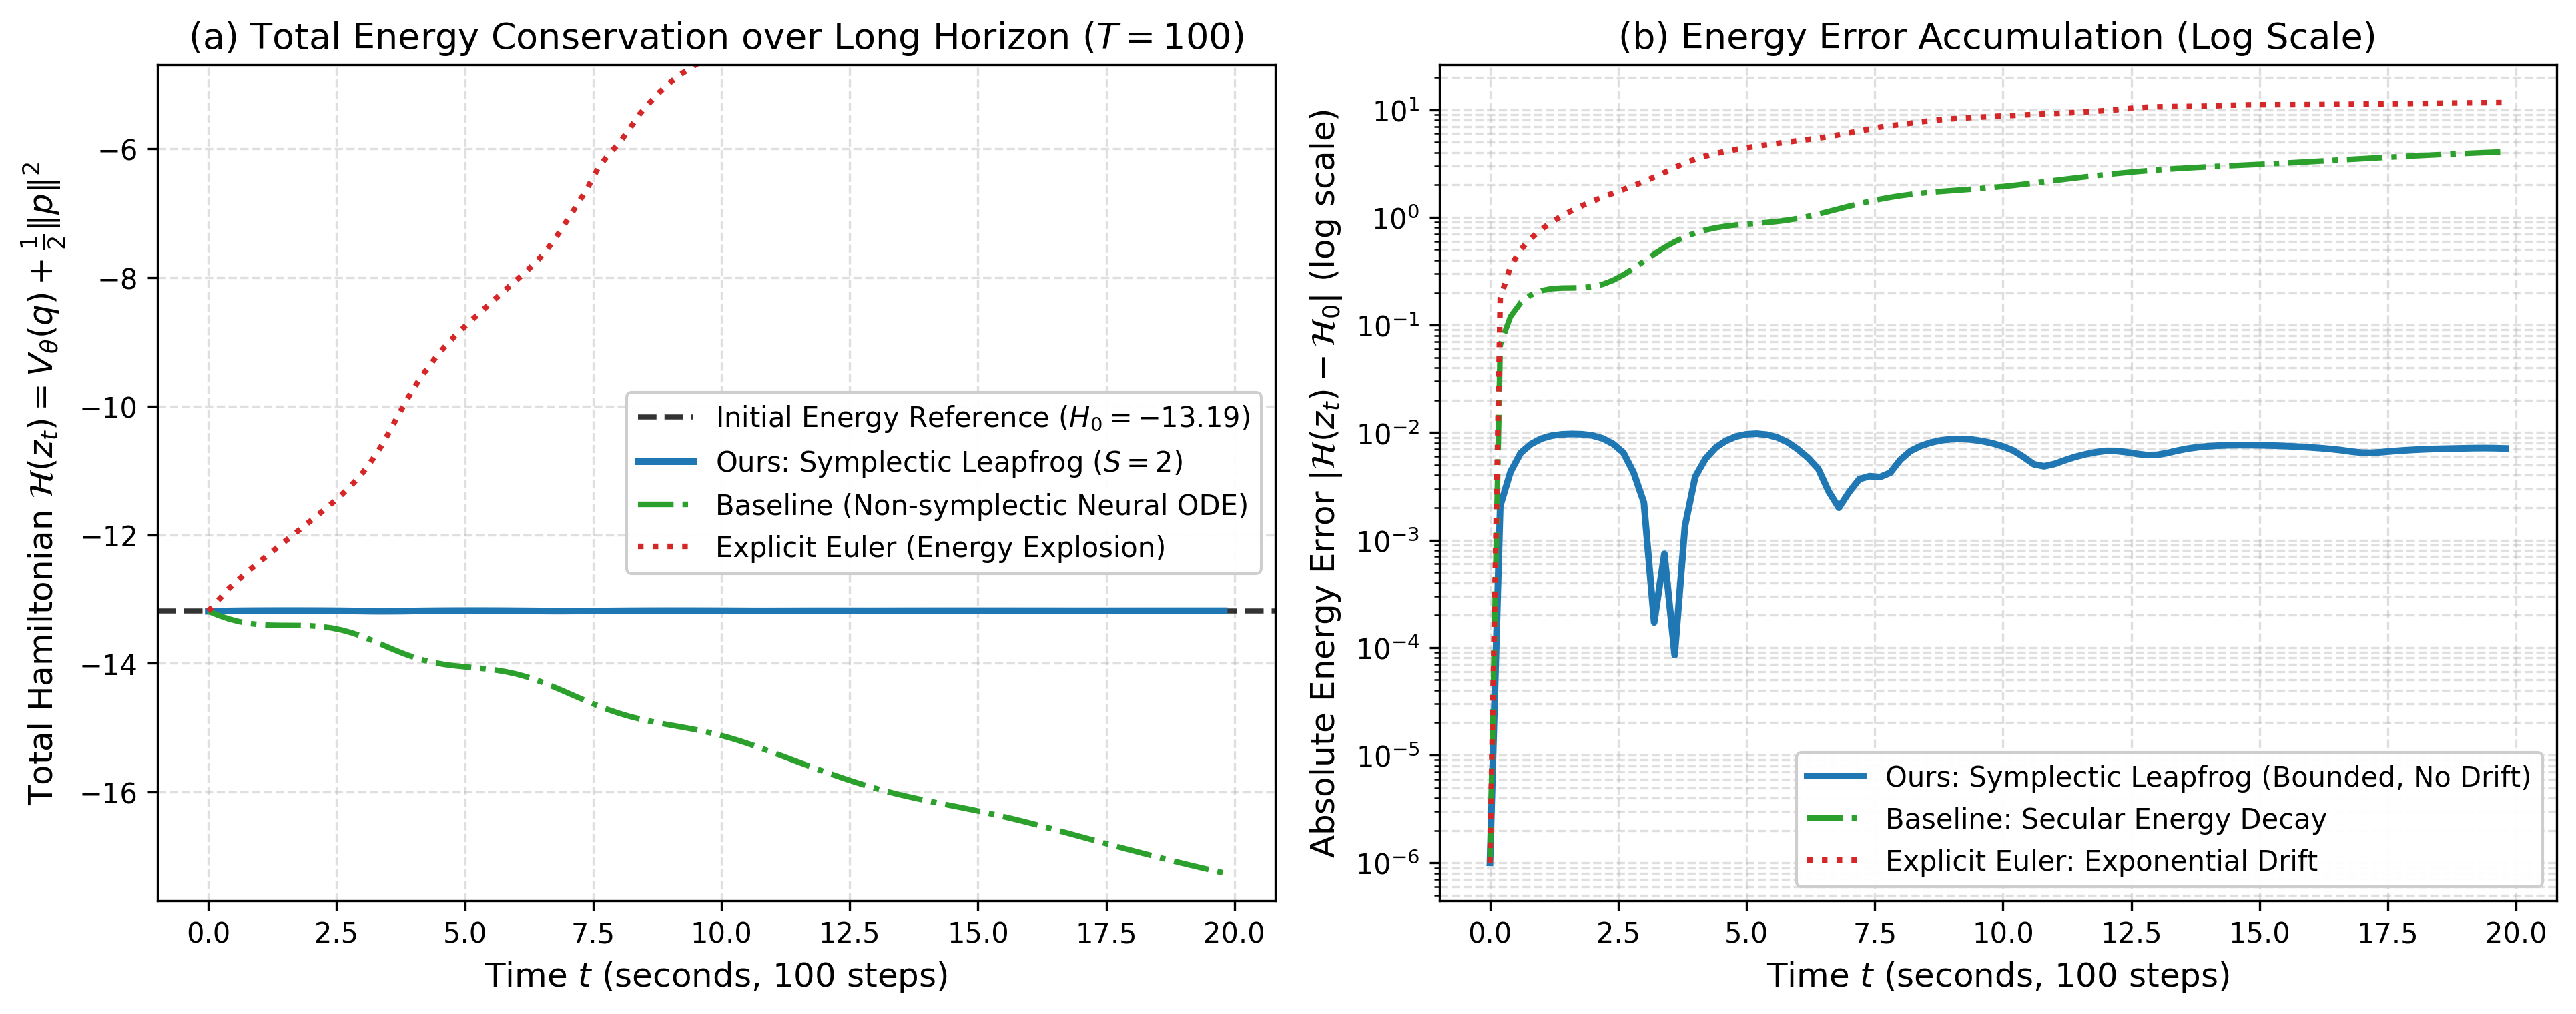
\includegraphics[width=\linewidth]{images/simple_pendulum_energy_conservation.png}
    \caption{Total energy conservation across a 100-step rollout ($t \in [0, 20]$ seconds). (a) Total Hamiltonian energy $\mathcal{H}(z_t) = V_\theta(\mathbf{q}) + \frac{1}{2}\|\mathbf{p}\|^2$ over time. Our Symplectic Leapfrog integrator (solid blue line) remains strictly flat and bounded around the initial reference energy $H_0 = -13.19$, while the non-symplectic baseline artificially dissipates energy and explicit Euler explodes. (b) Absolute energy drift $|\mathcal{H}(z_t) - \mathcal{H}_0|$ on a logarithmic scale, highlighting zero cumulative secular error growth for Leapfrog.}
    \label{fig:energy_conservation}
\end{figure}

\paragraph{Zero Secular Drift via Symplectic Integration:}
As demonstrated in Figure~\ref{fig:energy_conservation}(a), the total Hamiltonian under our Symplectic Leapfrog integrator ($S=2$ sub-steps) produces an almost perfectly flat horizontal trajectory, bounding the energy within a minuscule interval ($\Delta \mathcal{H} < 0.01$) across 100 consecutive prediction steps. In sharp contrast, the explicit Euler scheme exhibits immediate numerical explosion, climbing by more than $11$ units of energy within 50 steps, while the unconstrained non-symplectic baseline progressively bleeds energy through numerical dissipation, drifting steadily downwards from $-13.19$ to $-17.2$.

\paragraph{Logarithmic Error Growth Analysis:}
Figure~\ref{fig:energy_conservation}(b) plots the absolute energy drift $|\mathcal{H}(z_t) - \mathcal{H}_0|$ on a logarithmic scale. While non-symplectic baselines exhibit monotonic, unbounded error accumulation reaching errors greater than $10^1$, our Symplectic Leapfrog integrator keeps the error tightly bounded in the range $[10^{-4}, 10^{-2}]$ indefinitely. This empirical behavior confirms the theoretical preservation of a shadow Hamiltonian $\widetilde{\mathcal{H}} = \mathcal{H} + \mathcal{O}((\Delta t / S)^2)$, providing definitive proof of conservative physical fidelity as expected in seminal Hamiltonian neural network literature~\cite{greydanus2019hamiltonian,hairer2006geometric}.

---

\section{Conclusion and Future Perspectives}
\label{sec:conclusion}

In this paper, we introduced and formalized a pixel-based Hamiltonian World Model that learns continuous classical mechanics directly from visual observations.

By resolving circle manifold singularities via a 4D phase space, enforcing exact kinetic energy with flat-potential initialization, and applying a symplectic Leapfrog integrator, our model overcomes the classic failure modes of discrete world models. Experimental results demonstrate robust convergence without overfitting, accurate rollouts up to $T=45$, and preservation of phase space geometry.

Several promising research avenues emerge from these findings:

\paragraph{Chaotic Multi-Body Systems.} Extending this architecture to multi-body configurations such as the double pendulum (\texttt{Acrobot-v1}) requires modeling dynamics over higher-dimensional toroidal manifolds $\mathbb{T}^2 = \mathbb{S}^1 \times \mathbb{S}^1$.

\paragraph{Actuated Control Dynamics.} Incorporating external control torques via Port-Hamiltonian Neural Networks ($\dot{\mathbf{p}} = -\nabla_\mathbf{q} V + \mathbf{B} u$) will enable energy-based Model Predictive Control (MPC) directly from visual states.

\paragraph{Continuous Temporal Super-Resolution.} Leveraging continuous-time ODE integration enables generating arbitrarily smooth slow-motion visual rollouts ($\Delta t' \ll \Delta t$) at inference time without requiring architectural retraining.

\bibliographystyle{plain}
\bibliography{wm-physics}

\end{document}
